\documentclass[14pt]{mmcs_article}
\usepackage[russian]{babel}
\usepackage{amsmath, amsthm, amsfonts, amssymb}

\usepackage{paratype}

\usepackage{booktabs} % считаются наиболее профессионально выполненными
%\usepackage{ltablex}
%\newcolumntype {L} {>{---}l}

%%% Библиография

\usepackage{csquotes}        % Оформление списка литературы
\usepackage[
backend=biber,
hyperref=auto,
sorting=none, % сортировка в порядке встречаемости ссылок
language=auto,
citestyle=gost-numeric-min,
bibstyle=gost-numeric-min
]{biblatex}
\addbibresource{biblio.bib} % Файл с лит.источниками

\usepackage [toc,page] {appendix}
\renewcommand{\appendixtocname}{Приложения}
\renewcommand{\appendixpagename}{Приложения}

\usepackage{ifthen}
\newcounter{worktype}
\newcommand{\typeOfWork}[1]
{
	\setcounter{worktype}{#1}
}

% ВНИМАНИЕ!
% Укажите тип работы: 0 - курсовая, 1 - бак., 2 - маг.,
% 3 - бакалаврская с главами.
\typeOfWork{2}
% Настройка величины отступа в списке
\ifthenelse{\value{worktype} < 2}{%
	\defbibenvironment{bibliography}
	{\list
		{\printtext[labelnumberwidth]{%
				\printfield{prefixnumber}%
				\printfield{labelnumber}}}
		{\setlength{\labelwidth}{\labelnumberwidth}%
			\setlength{\leftmargin}{\labelwidth}%
			\setlength{\labelsep}{\dimexpr\MyIndent-\labelwidth\relax}% <----- default is \biblabelsep
			\addtolength{\leftmargin}{\labelsep}%
			\setlength{\itemsep}{\bibitemsep}%
			\setlength{\parsep}{\bibparsep}}%
		\renewcommand*{\makelabel}[1]{\hss##1}}
	{\endlist}
	{\item}
}{}

%\graphicspath{{images/}}%путь к рисункам

\begin{document}

% Титульные листы
% раскомментировать требуемое
%\include{Titul3k} % для курсовой
%\include{TitulBak}% для работы бакалавра
%см. РЕКОМЕНДАЦИИ ПО ОФОРМЛЕНИЮ
%И ПРЕДСТАВЛЕНИЮ КУРСОВЫХ И ВЫПУСКНЫХ %КВАЛИФИКАЦИОННЫХ РАБОТ СТУДЕНТОВ ИНСТИТУТА %МАТЕМАТИКИ, МЕХАНИКИ И КОМПЬЮТЕРНЫХ НАУК


% ----------------------------------
% Внимание!
% Изменяйте только строки, перед которыми стоят знаки комментариев
% ----------------------------------

\thispagestyle{empty}
\begin{singlespacing} 
\begin{center}

МИНОБРНАУКИ РОССИИ\\ [12pt]
Федеральное государственное автономное образовательное\\
учреждение высшего образования\\
<<Южный федеральный университет>>

\vspace{\baselineskip}
Институт математики, механики\\
и компьютерных наук им.~И.\,И.~Воровича


\vfill
% Фамилия Имя Отчество студента
\textbf{Коваленко Алексей Сергеевич}

\vspace{15mm}
%НАЗВАНИЕ РАБОТЫ должно полностью соответствовать 
% приказу по ЮФУ (для выпускных квалификационных работ)
{\bf Обучение шумоподавляющих автоэнкодеров без чистых данных }

\vspace{15mm}
ВЫПУСКНАЯ КВАЛИФИКАЦИОННАЯ РАБОТА\\
по направлению подготовки\\
% Направление обучения 
02.04.02~-- Фундаментальная информатика и информационные технологии,\\
<<Разработка компьютерных игр и мобильных приложений>>

\vspace{10mm}
\textbf{Научный руководитель~--}\\
% указать данные о руководителе
% должность, степень, звание Фамилия Имя Отчество
 доц., к.\,т.\,н. Демяненко Яна Михайловна

\vspace{7mm}
\textbf{Рецензент~--}\\
% указать данные о рецензенте
% должность, степень, звание Фамилия Имя Отчество
доц., к.\,ф.-м.\,н. Гуда Сергей Александрович


\vspace{15mm}

\noindent
% указать Фамилию и инициалы руководителя
% образовательной программыы
\begin{flushleft}
Допущено к защите:\\
руководитель \\
образовательной программы \underline{\hspace*{50mm}} Демяненко Я.\,М.
\end{flushleft}




\vfill
% год!
Ростов-на-Дону -- 2020

\end{center} 

\singlespacing
\end{singlespacing}% для работы магистра

\renewcommand{\contentsname}{Оглавление}

\tableofcontents

%=======================
\newpage
\addcontentsline{toc}{section}{Постановка задачи}

\section*{Постановка задачи}


В постановке задачи коротко (по пунктам) указывается, что необходимо сделать в рамках работы. Раздел <<Постановка задачи>> должен соответствовать заданию на курсовую или выпускную квалификационную работу, подписанному научным руководителем.


\newpage
\addcontentsline{toc}{section}{Введение}
\section*{Введение}

Шумоподавление является часто встречаемой задачей в области компьютерного зрения. Так как любое изображение, полученное из картины реального мира является дискретным представлением непрерывного аналогового сигнала, то в нём будет присутствовать шум. Изначально шум появляется у полезного сигнала из-за погрешностей приёма оптического излучения фотоидами, данное явление изложено в книге Fundamentals of linear electronics~\autocite{HardwareImageNoise}. Затем к данному искажённому сигналу добавляются потери при процессе дискретизации. Действие шума на изображения можно легко увидеть на примере изображения \ref{fig:noise_compration}, на правой части изображения приводится пример фотографии, снятой при более благоприятных условиях, при которых фотосенсор цифровой камеры порождает меньше шума, чем на фотографии слева. 

\begin{figure}[h]
	\centering
	\includegraphics[width=\textwidth]{img/Noise_Comparison}
	\caption{Пример зашумленного изображения.}
	\label{fig:noise_compration}
\end{figure}

Также существуют изображения, полученные не только с фотосенсоров. Примером можно привести рентгенографию, широко используемую во многих областях, таких как медицина, процессы производства и эксплуатации, криминалистика, реставрация и экспертиза художественных ценностей. Существует два варианта получения цифрового изображения рентгенографии, это оцифровка уже существующего рентгеновского снимка, и использование технологии цифровой рентгенографии, при которой сразу идет цифровая обработка получаемого рентгеновского изображения. Оба данных метода подвержены наличию шума на получаемом цифровом изображении, в большей мере шум преобладает на изображених, получаемых первым способом, так как идёт дополнительное наложение шума сканирующим устройством. Пример подобного шума проиллюстрирован на изображении \ref{fig:reng_scan}. Аналогичная ситуация наблюдается и с снимками в области радиографического контроля сварных соединений, пример проиллюстрирован на изображении \ref{fig:reg_met_scan}.

\begin{figure}[h]
	\centering
	\includegraphics[width=\textwidth]{img/reng_scan}
	\caption{Сканированный рентгеновский снимок грудной клетки человека.}
	\label{fig:reng_scan}
\end{figure}

\begin{figure}[h]
	\centering
	\includegraphics[width=\textwidth]{img/reng_met_scan}
	\caption{Цифровой рентгеновский снимок сварного соединения.}
	\label{fig:reg_met_scan}
\end{figure}

Помимо рентгенографии в обработке медицинских изображений потребность в избавлении полезного сигнала от шума встречаются и в других методах диагностики и визуализации, таких как цифровая реконструкция компьютерной томографии, магнитно-резонансной томографии и других. Потребность в шумоподавлении на медицинских цифровых изображениях изложена в работе~\autocite{MedicalImagesProcessing}.

На данный момент с развитием технологий глубокого обучения и построения глубоких архитектур сверточных нейронных сетей, такие архитектуры применяются к решению широкого ряда задач в области обработки и анализа изображений. Существует три подхода к обучению нейронных сетей: обучение с учителем, обучение без учителя и обучение с подкреплением. Если рассматривать близкие задачи к шумоподавлению с точки зрения построения шаблона обучения сети, это задача увеличения разрешения изображения с помощью нейронных сетей~\autocite{SuperResolutuion:journals/corr/abs-1807-02758} и задача восстановления изображения~\autocite{ImageReconstruction}. Для решения данных задач нейросетевые архитектуры обучаются с помощью подхода обучения с учителем~\autocite{SupervisedLearningReview}. При процессе обучения таких архитектур в качестве входных данных выступают сжатые варианты изображений, подаваемых, как ожидаемые при предсказании сети. Если рассматривать в данном контексте обучение для задачи классификации, то на вход сети необходимо подавать изображение с присутствующем на нём шумом, и обучать сеть предсказывать уже само чистое изображение без шума. 

Все перечисленные способы в этом разделе получения цифрового изображения объединяет один недостаток, это невозможность получения чистого изображения без шума для обучения шумоподавляющей нейронной сети. В данной работе рассматривается подход к построению архитектуры шумоподавляющей нейронной сети и построения обучающего процесса, основанного на методе обучения без учителя (неконтролируемое обучение).


%=======================
\newpage

\section{Детальная постановка задачи}\label{sec:set_task}
Пусть имеется изображение в формате непрерывного сигнала, полученного с АЦП об сигналах матрицы фотосенсора фиксированного цифрового устройства в момент времени $t$ (DNG формат~\autocite{DNG}):
\begin{equation}\label{eq:signal}
S(t)
\end{equation}

Сигнал $S(t)$~(\ref{eq:signal}) состоит из полезного сигнала $G(t)$ и шума $r(t)$, порождаемым фотосенсором:
\begin{equation}\label{eq:signal_decomposition}
S(t)\ =\ G(t)\ +\ r(t)
\end{equation}

При применении преобразования сырого сигнала $S(t)$ к трехмерному дискретному изображению в цветовой схеме RGB получаем матрицу изображения  $\tilde{I}$, с влиянием шума квантования при округлении сигнала при его дискретизации. Подход преобразования $p$ описан в работе Processing RAW Images in MATLAB~\autocite{RAWtoRGB}.
\begin{eqnarray}\label{eq:raw_image_matrix}
\tilde{I}_{i,j} = p(S(t))_{i, j}\ +\ q,\ q  \sim \mathcal{N}(-\frac{1}{2}, \frac{1}{12})\ \text{,}
\end{eqnarray}
где $q$, это шум квантования, семплируемый из нормального распределения с параметрами $\mathcal{N}(-\frac{Q}{2}, \frac{Q}{12})$ при шаге квантования $Q\ =\ 1$, более подробно можно ознакомиться с этим в главе Оценки ошибок (шумов) квантования выходного сигнала в цифровом фильтре из книги Цифровая обработка сигналов~\autocite{DSP}.

Для упрощения постановки задачи будем полагать, что матрица изображения $\tilde{I}$ состоит из суммы изображения, полученного из преобразования чистого (полезного) сигнала $G(t)$~(\ref{eq:signal_decomposition}) в матрицу $I$ и шума $\alpha$, полученного из случайного распределения $\mathbb{P}$, так как появление шума $r(t)$~(\ref{eq:raw_image_matrix}) можно считать абсолютно случайным процессом.
\begin{equation}\label{eq:matrix_def}
\tilde{I}\ =\ I\ +\ \alpha,\ \alpha \sim \mathbb{P}
\end{equation}

Таким образом, имея серию из $N$ изображений одной и той же сцены, снятых в разный момент времени $t$ имеем следующую выборку:
\begin{equation}\label{eq:collection}
\{\tilde{I}_k\}_{k=1}^{N}\text{ , где }\tilde{I_k}\ =\  I\ +\ \alpha_k,\ \alpha_k \sim \mathbb{P}
\end{equation}
Причём для каждого элемента из набора $\tilde{I}_k$ компонента $I$ является одним и тем же значением, так как при съёмке одной сцены полезный сигнал $G(t)$~(\ref{eq:signal_decomposition}) остаётся неизменным.

Целью данной работы является построение с помощью нейронной сети приближения отображения $\phi: \mathbb{R}^n \longrightarrow \mathbb{R}^n$, обладающим следующим свойством:
\begin{equation}\label{eq:main_property}
\forall \tilde{I} \in \{\tilde{I}_k\}_{k=1}^{N} \Longrightarrow \phi(\tilde{I}) = I 
\end{equation}
Для построения приближения отображения $\phi$, нейронная сеть $f$ будет обучаться решать следующую задачу оптимизации:
\begin{eqnarray}\label{eq:main_min_task}
\min_{\mathnormal{w}} \Arrowvert f(\tilde{I}, \mathnormal{w}) - I \Arrowvert_{L_2}\text{ ,}
\end{eqnarray}
где $\mathnormal{w}$ - параметры сети $f$, $L_2$ - евклидова норма~\autocite{Haykin}.


\section{Анализируемые данные}\label{sec:our_data}
\subsection{Сбор данных}
Так как в данной работе поставлена задача подавления шума у сигнала с заданного сенсора, то изображения для проведения исследования были получены с помощью фиксированного устройства, \textit{Apple iPhone X}, имеющего камеру, состоящую из двух сенсоров, с характеристиками, приведенными в таблицах~\ref{tab:cam1} и~\ref{tab:cam2}.

\begin{table}[h!]
	\centering
	\caption{\label{tab:cam1}Характеристики первого сенсора}
	\begin{tabular}{llr}
		% \toprule
		\hline
		Характеристика  & Значение    & Единица измерения \\
		% \midrule
		\hline
		Разрешение & 12    & $MP$  \\
		Апертура & f/1.8 & \\
		Фокусное расстояние & 28 & $mm$ \\
		Размер сенсора & 1/3" & \\
		Размер пикселя & 1.22 & $\mu m$ \\
		Стабилизация изображения & OIS & \\
		% \bottomrule
		\hline
	\end{tabular}
\end{table}

\begin{table}[h!]
	\centering
	\caption{\label{tab:cam2}Характеристики второго сенсора}
	\begin{tabular}{llr}
		% \toprule
		\hline
		Характеристика  & Значение    & Единица измерения \\
		% \midrule
		\hline
		Разрешение & 12    & $MP$  \\
		Апертура & f/2.4 & \\
		Фокусное расстояние & 52 & $mm$ \\
		Размер сенсора & 1/3.4" & \\
		Размер пикселя & 1.0 & $\mu m$ \\
		Стабилизация изображения & OIS & \\
		 %\bottomrule
		 \hline
	\end{tabular}
\end{table}

С данного устройства были сделаны серии изображений семи сцен с различным освещением и цветовым наполнением. Данные серии получены стандартными средствами для съёмки на устройстве. При такой съемке автоматически применяются алгоритмы улучшения кадра на устройстве, в том числе и подавление шума. Данные алгоритмы являются коммерческой тайной компании Apple~\autocite{APPLElink}. Под сценой подразумевается съёмка неизменяемой картины реального мира, получая матрицу~(\ref{eq:matrix_def}). Для этого устройство фиксировалось на штативе в неподвижном состоянии  и запуск процесса съёмки кадра производился  с беспроводного устройства, тем самым получая набор изображений $\{\tilde{I}^q_k\}_{k=1}^{N}$~(\ref{eq:collection}), где $q$ - порядковый номер снимаемой сцены. Для каждой сцены при съемке были зафиксированны значения ISO, фокуса и цветовой температуры. 

% 95 фотографий
Каждая сцена содержит в среднем по $14$ фотографий, суммарное количество кадров из всех наборов составляет $95$ изображений.


Так как стандартные средства для съёмки не позволяют получать RAW (изображение с сырого сигнала АЦП~(\ref{eq:signal})) изображение, то были произведены съёмки дополнительных сцен с использованием стороннего программного обеспечения, позволяющего получать <<сырые>>  кадры в формате TIFF~\autocite{TIFFArticle}: Simple Raw camera~\autocite{RAWCamera}. С помощью данного приложения были сняты серии трёх дополнительных сцен. Данные серии содержат суммарно $30$ изображений, ровно по $10$ кадров в каждой серии.

Максимальное количество изображений в одной серии ограничено $20$-ю кадрами, так как при продолжении процесса съёмки фотосенсор нагревается и из-за теплового воздействия появляются дополнительные искажения сигнала, из-за которых теряется попиксельное соответствие кадров в серии между собой.

В итоге получается набор данных, состоящий из $125$ изображений, снятых на один сенсор. Визуальное различие шума на изображениях, полученных разными подходами можно рассмотреть на рисунке~\ref{fig:noise_comprasion}.

Также для сравнения результатов были сделаны 6 серий, снятых следующей web камерой~\autocite{WebCam} в разрешении $1920\times1080$. Снимались видеозаписи короткой длительности и разбивались на кадры с помощью библиотеки FFmpeg~\autocite{FFMPEG}. Суммарное количество кадров в данных сериях составило $811$.

\begin{figure}[h]
	\centering
	\includegraphics[width=\textwidth]{img/noise_comprasion}
	\caption{Сравнение получаемого шума на изображении, снятого стандартными средствами устройства (слева) и RAW изображения (справа)}
	\label{fig:noise_comprasion}
\end{figure}


\subsection{Анализ собранных данных}

Во время процесса съемки при нагреве фотосенсора могут происходить незначительные искажения кадра. Или также возможны незаметные смещения устройства при съемке, а также смена внешних условий, таких как освещение или движение объектов в кадре. Для собираемого набора изображений сдвиг более чем на один пиксель между кадрами одной серии уже критичен.

Для анализа качества полученных серий изображений были построены распределения $e^q$~(\ref{eq:series_distribution}) отклонений каждого изображения от усредненного по всем изображениям из серии $\hat{I}^q$~(\ref{eq:mean_image}) по евклидовой метрике.
\begin{eqnarray}\label{eq:mean_image}
\hat{I}^q_{i,j}\ =\ \frac{\sum_{k}\tilde{I}^q_{k\ i,j}}{N}\text{, где }N\text{ количество кадров в выборке }q
\end{eqnarray}

\begin{eqnarray}\label{eq:series_distribution}
e^q_k\ =\ \Arrowvert \hat{I}^q - \tilde{I}^q_k \Arrowvert_{L_2}
\end{eqnarray}
Дополнительно производится нормировка выборки по метрике $L_1$:
$$e^q_k\ =\ \frac{e^q_k}{\sum_{i}(e^q_i)}$$

Далее по значениям выборки $e^q$~(\ref{eq:series_distribution}) строятся графики плотности нормального распределения $\mathcal{N}(\mu, \sigma)$ с параметрами:
\begin{eqnarray}\label{eq:mean_and_std}
\mu^q = \mu(e^q),\ \sigma^q = \sigma(e^q)
\end{eqnarray}

Таким образом математическое ожидание $\mu^q$~(\ref{eq:mean_and_std}) показывает насколько усредненное изображение $\hat{I}^q$~(\ref{eq:mean_image}) близко к изображению, теоретически, получаемому из чистого сигнала $I^q$~(\ref{eq:collection}): 
\begin{eqnarray}\label{eq:mean_image_approximation}
\hat{I}^q \xrightarrow[\mu^q \rightarrow 0]{} I^q
\end{eqnarray}

А также, чем ближе к $0$ значение среднеквадратичного отклонения выборки $\sigma^q$~(\ref{eq:mean_and_std}), тем на большем количестве изображений из серии присутствует сигнал $G(t)$~(\ref{eq:signal_decomposition}), зафиксированный в момент времени $t = t_0$, то есть насколько сцена неизменна между кадрами.

Графики распределений для серий, снятых стандартными средствами устройства \textit{Apple iPhone X} изображен на рисунке~\ref{fig:distribuion_after_apple_denoising}. Из графиков можно увидеть, что чем больше размер серии, тем ближе усредненное изображение к чистому.

\begin{figure}[H]
	\centering
	\includegraphics[width=\textwidth]{img/series_apple_denoising_deviation_comparison}
	\caption{Графики плотностей нормальных распределений для серий, снятых стандартными средствами устройства \textit{Apple iPhone X}}
	\label{fig:distribuion_after_apple_denoising}
\end{figure}


Рассматриваемый параметр $\sigma$~(\ref{eq:mean_and_std}) сильно зависит не только от движения объектов на снимаемой сцене, но и от уровня освещения. Сдвиг объектив особо критичен, так как обученная нейросеть на такой выборке будет размывать результирующие изображение. Сравнение усредненного изображения, имеющего сдвиг сцены с изображением, полученным из усреднения кадров статичной сцены изображено на рисунке~\ref{fig:deviations_comparision}. 

\begin{figure}[H]
	\centering
	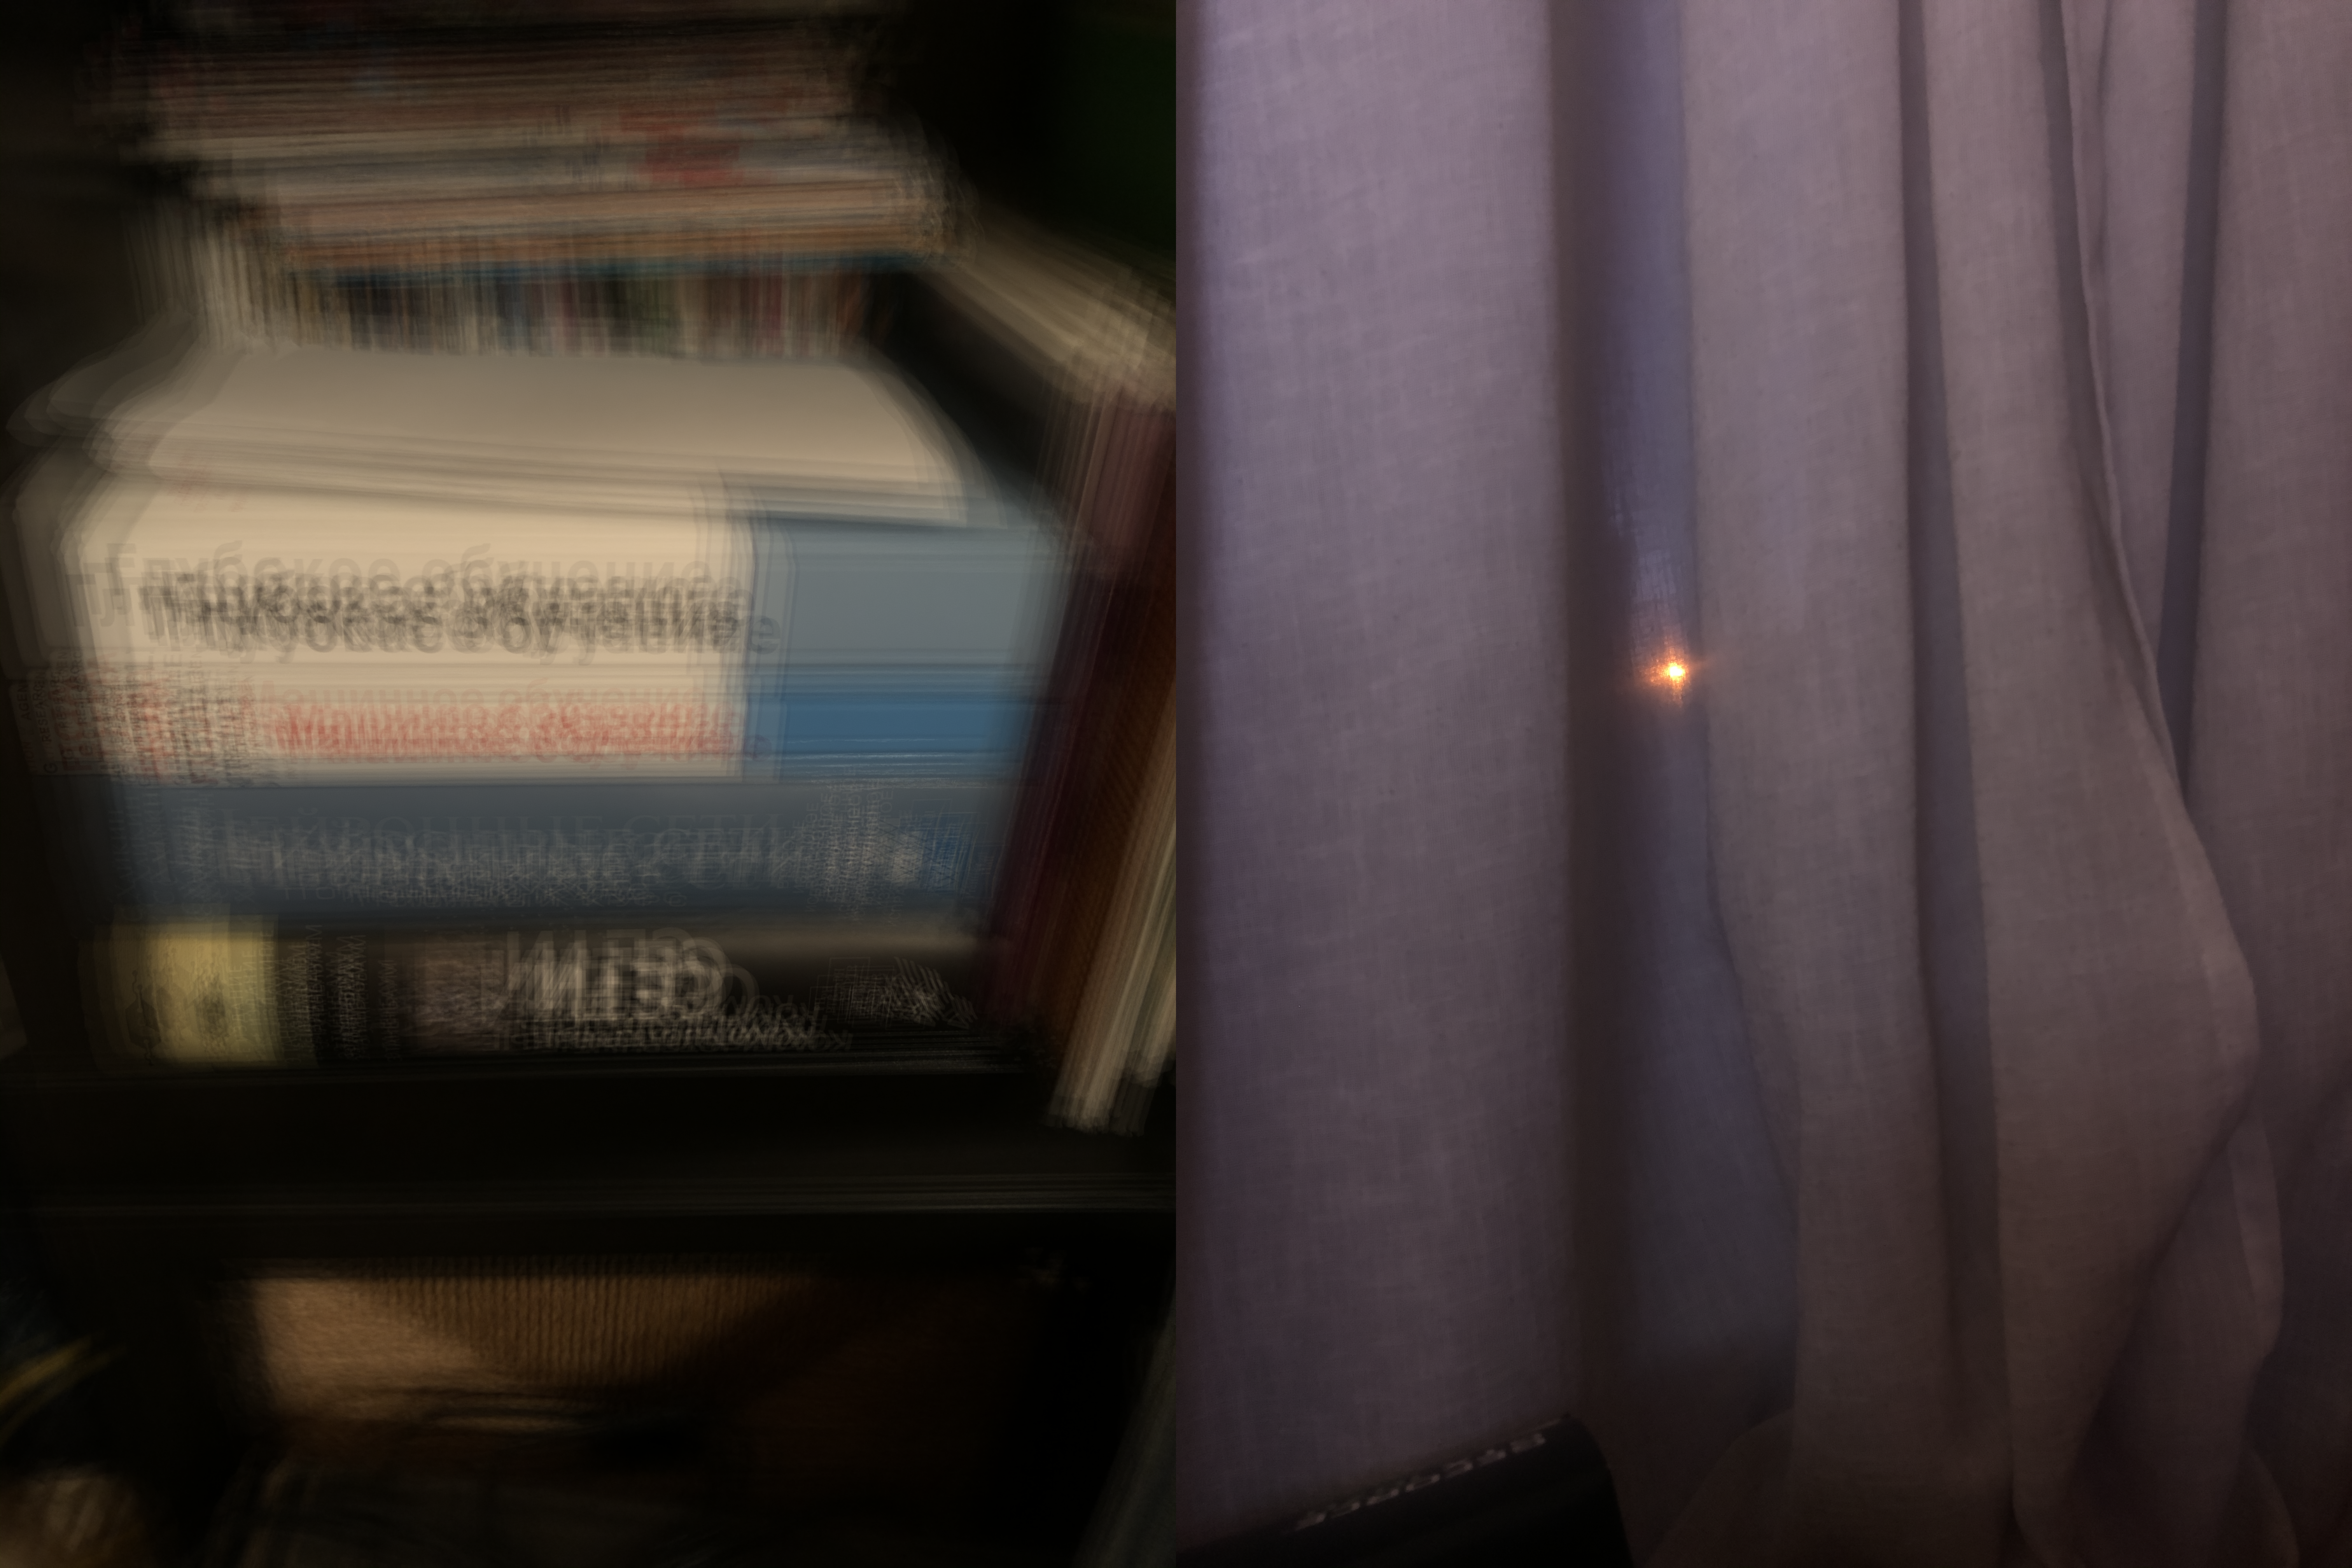
\includegraphics[width=\textwidth]{img/incorrect_and_correct_comparison}
	\caption{Для среднего изображения серии слева $\sigma = 0.00891$, для среднего изображения серии справа $\sigma = 0.00272$}
	\label{fig:deviations_comparision}
\end{figure}

Также большое значение отклонения $\sigma$~(\ref{eq:mean_and_std}), полученное из-за сильного изменения освещения при съемке также неблагоприятно скажется на качестве обучения нейронной сети, так как нейронная сеть, обученная на таких сериях, не сможет корректно предсказывать цветовую гамму результирующего изображения. Пример зависимости параметра отклонения от уровня освещения снимаемой сцены при естественном освещении изображен на рисунке~\ref{fig:hists_comparision}. Из данного примера  можно заметить, что незначительные отклонения в освещении, различимые по небольшим отличиям в цветовых гистограммах изображений из серии сильно влияют на параметр $\sigma$~(\ref{eq:mean_and_std}), и для данной статичной сцены данный параметр близок к значению, получаемому у сцены с сильным сдвигом~\ref{fig:deviations_comparision}.


\begin{figure}[H]
	\centering
	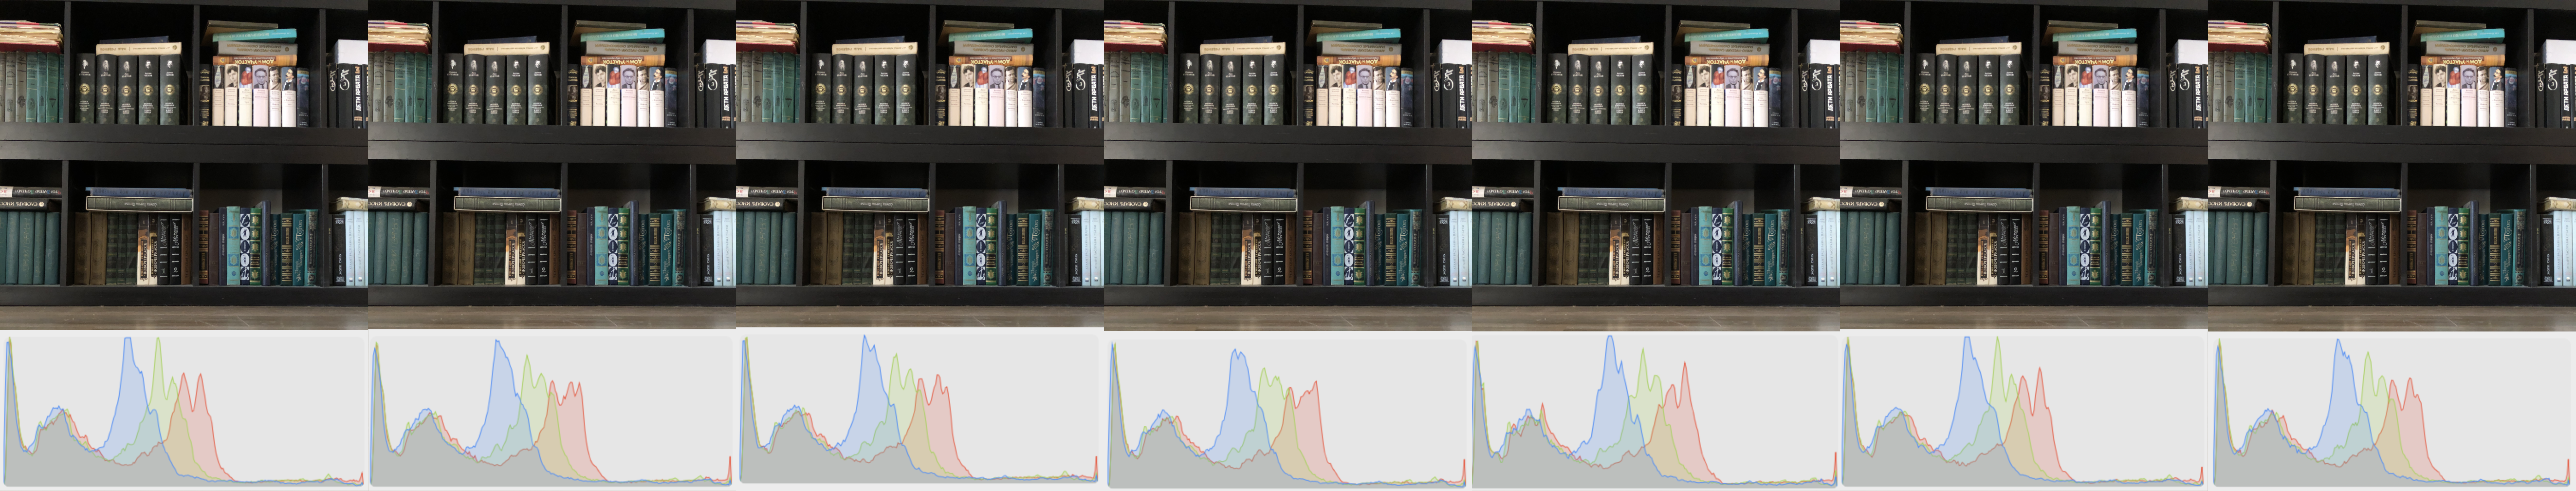
\includegraphics[width=\textwidth]{img/imgs_8_series_stack_image}
	\caption{Серия изображений с цветовыми гистограммами, параметр $\sigma$ данной серии равен $0.00608$ }
	\label{fig:hists_comparision}
\end{figure}

Для остальных условий съемки аналогичным образом были построены графики с распределениями, изображенные на рисунках~\ref{fig:distribuion_real_noise},~\ref{fig:distribuion_real_noise_good_condition} и~\ref{fig:distribuion_webcam}. Серии, полученные с web камеры содержат относительно большое количество кадров каждой сцены (в среднем по $135$) и не подвергаются искажениям из-за нагрева сенсора за счет большего шага дискретизации изображения реального мира (меньшего разрешения).

\begin{figure}[H]
	\centering
	\includegraphics[width=\textwidth]{img/night_condition_series_real_noise_iphone_deviation_comparison}
	\caption{Графики плотностей нормальных распределений для серий, снятых при условиях плохого искусственного освещения с помощью приложения~\autocite{RAWCamera}}
	\label{fig:distribuion_real_noise}
\end{figure}


\begin{figure}[H]
	\centering
	\includegraphics[width=\textwidth]{img/good_condition_series_real_noise_iphone_deviation_comparison}
	\caption{Графики плотностей нормальных распределений для серий, снятых при условиях естественного освещения с помощью приложения~\autocite{RAWCamera}}
	\label{fig:distribuion_real_noise_good_condition}
\end{figure}

\begin{figure}[H]
	\centering
	\includegraphics[width=\textwidth]{img/series_webcam_deviation_comparison}
	\caption{Графики плотностей нормальных распределений для серий, снятых при разных условиях освещения с помощью web камеры~\autocite{WebCam}}
	\label{fig:distribuion_webcam}
\end{figure}


При выборе данных для обучения нейронных сетей подавляющих шум на изображении задается условие, что параметр $\sigma$~(\ref{eq:mean_and_std}) не должен превышать значения $0.007$

\section{Существующие решения}
\subsection{Подходы, не использующие нейронные сети}

\subsubsection{Гауссовское размытие}
Одним из самых распространённых подходов подавления шума на изображении является применение гауссовского размытия. Оно заключается в свертке изображения с ядром, полученным следующей функцией:
\begin{eqnarray}\label{eq:gauss_kernel_function}
g(x, y)\ =\ A \ast e^{-\frac{x^2 + y^2}{\sigma^2}}
\end{eqnarray}
где параметр $\sigma$ задаёт степень размытия, а параметр $A$ обеспечивает нормировку. Более детально данный подход описан в работе~\autocite{GaussianBilinear}.

Основным достоинством данного подхода является простота реализации алгоритма и быстрая скорость работы. Также данный подход имеет реализацию во всех популярных библиотеках для обработки изображений на языках программирования Python и C/C++, таких как OpenCV~\autocite{OpenCVLib}.

Если рассматривать данный подход применительно к анализируемым данным, то подход справляется только с шумом, полученным после обработки стандартными средствами съемки устройства, но и при этом можно заметить размытие кадра уже с использованием свертки размера $5$. Результат можно увидеть на рисунке~\ref{fig:apple_noise_gauss_comparison}. Если рассматривать применительно к сырым RAW изображениям, то и при сильном размытии остается заметный шум и при этом сильно размывается изображением. Результат такого применения можно увидеть на изображении~\ref{fig:real_noise_gauss_comparison}. Для получения данных результатов использовалась реализация из библиотеки OpenCV~\autocite{OpenCVLib}.

\begin{figure}[H]
	\centering
	\includegraphics[width=\textwidth]{img/apple_noise_gaussian_params_comparison}
	\caption{Результат работы гауссовского размытия на изображении со стандартной обработкой телефона. Слева направо: оригинальное изображение, с применением размытия с параметром $\sigma = 1$ и размером ядра $5$, с применением размытия с параметром $\sigma = 2$ и размером ядра $9$}
	\label{fig:apple_noise_gauss_comparison}
\end{figure}

\begin{figure}[H]
	\centering
	\includegraphics[width=\textwidth]{img/real_noise_gaussian_params_comparison}
	\caption{Результат работы гауссовского размытия на сыром (RAW) изображении. Слева направо: оригинальное изображение, с применением размытия с параметром $\sigma = 1$ и размером ядра $5$, с применением размытия с параметром $\sigma = 2$ и размером ядра $9$}
	\label{fig:real_noise_gauss_comparison}
\end{figure}

\subsubsection{Медианный фильтр}

Медианный фильтр реализуется следующим образом: для каждого пикселя в некотором окружении окна, заданного размера $d,\ d\ mod\ 2 == 1$ находится медианное значение данного набора пикселей и присваивается текущему. Также индекс медианного пикселя для рассматриваемого пикселя $p$ можно представить в следующем виде:
\begin{equation}
median\ index\ =\ \arg\ \min_{p_i \in P} \sum_{p_j \in P} \Arrowvert p_i - p_j \Arrowvert_{L_1}
\end{equation}
$$P = \{I_{i, j}\}_ {(i - i_p)^2 + (j - j_p)^2 \le d^2},\ \text{где }i_p, j_p\text{ координаты пикселя }p$$

Результат применения реализации данного метода из библиотеки OpenCV~\autocite{OpenCVLib} на анализируемых данных изображен на рисунке~\ref{fig:medianblur_comparison}. Эффекта подавления шума на обоих примерах удается при значении параметра $d = 15$, но при этом изображения имеют потерю высоких частот. Подробно данный метод описан в работе~\autocite{MedianBluPaper}. 

\begin{figure}[H]
	\centering
	\includegraphics[width=\textwidth]{img/medianfilter_comparison}
	\caption{Применение медианного фильтра для обработанного стандартными средствами изображения (сверху) и чистого RAW изображения (снизу)}
	\label{fig:medianblur_comparison}
\end{figure}

\subsubsection{Двустороннее сглаживание}
Двусторонняя фильтрация (Bilateral filtering) сглаживает изображения при сохранении краев посредством нелинейной комбинации соседних значений изображения. Данный подход описан в работе~\autocite{BilateralPaper}. Данный метод подавления шума, как и предыдущие является широко распространенным и имеет реализации в большинстве библиотек для работы с изображениями. 

Применяя данный алгоритм к анализируемым данным, можно увидеть, что он хорошо справляется с шумом, содержащимся в сырых RAW изображениях, но при этом теряются высокие частоты изображения, что приводит к размытию линий в нижней левой части кадра из примера, изображенного на рисунке~\ref{fig:bilinear_comparison}. Применение данного алгоритма к предобработанным стандартными средствами устройства изображениям не дает ощутимого результата, это можно увидеть на изображении~\ref{fig:bilinear_comparison}. В обоих случаях использовалась реализация из библиотеки OpenCV~\autocite{OpenCVLib} с параметром радиуса $r = 15$.

\begin{figure}[H]
	\centering
	\includegraphics[width=\textwidth]{img/bilinear_comparison}
	\caption{Применение метода двусторонней фильтрации для обработанного стандартными средствами изображения (сверху) и чистого RAW изображения (снизу)}
	\label{fig:bilinear_comparison}
\end{figure}

\subsubsection{Non-Local Means Denoising}
Метод нелокального подавления шума для окна фиксированного размера $d$ заданного пикселя $p$ ищет похожие части на рассматриваемом изображении и заменяет пиксель $p$ усреднением всех похожих частей изображения. Данный метод подробно описан в работе~\autocite{NonLocalMeansDenoising}.

Сравнительно методов подавления шума, рассмотренных выше, данный фильтр имеет более высокую вычислительную сложность, но при этом и дает лучший результат. Результат применения данного подхода, реализованного в библиотеке OpenCV~\autocite{OpenCVLib} с размером окна $10$ к анализируемым данным изображен на рисунке~\ref{fig:nlmdenoising_comparison}. Данный подход хорошо подавляет шум на изображении, но при этом появляются артефакты и размытия в некоторых областях.

\begin{figure}[H]
	\centering
	\includegraphics[width=\textwidth]{img/nlmdenoising_comparison}
	\caption{Применение метода нелокального подавления шума для обработанного стандартными средствами изображения (сверху) и чистого RAW изображения (снизу)}
	\label{fig:nlmdenoising_comparison}
\end{figure}

\subsection{Подходы, основанные на нейронных  сетях}

\subsubsection{Полносверточные сети обучаемые с учителем}

Одним из значимых подходов в области подавления шума с использованием нейронных сетей является подход, изложенный авторами в работе Beyond a Gaussian Denoiser: Residual Learning of Deep CNN for Image Denoising~\autocite{DeepPrior}. Проводя своё исследование авторы опираются на большое количество подходов шумоподавления с помощью применения нейронных сетей. В данной работе рассматривается обучения сети при наличии изображений без шумового сигнала к соответствующим зашумленным экземплярам данных. Работу данной сети авторы демонстрируют на изображениях, к которым был добавлен псевдослучайный шум.

Не удалось повторить эксперименты авторов данной работы применительно к анализируемым данным, так как данная архитектура требует передачи на вход изображения целиком и это требует чрезмерного количества видеопамяти. Данная особенность является главным недостатком такого подхода. Работу данного подхода, на примере, предоставленным авторами можно видеть на рисунке~\ref{fig:deep_prior_authors_example}.

\begin{figure}[H]
	\centering
	\includegraphics[width=\textwidth]{img/deep_prior_res}
	\caption{Результаты работы подхода из работы~\autocite{DeepPrior}, на данных, предоставленными авторами. Слева - пример с добавлением псевдослучайного шума из нормального распределения, по центру - результат работы сети, справа - оригинальное изображение}
	\label{fig:deep_prior_authors_example}
\end{figure}

\subsubsection{Полносверточные сети обучаемые без учителя}

Авторы работы Noise2Noise: Learning Image Restoration without Clean Data~\autocite{Noise2NoisePaper} рассматривают подход обучения сверточных нейронных сетей опираясь только на данные, содержащие шум. Данная работа вносит весомый вклад в область обучения сетей, подавляющих шум. Почти все авторы данной работы являются инженерами в компании Nvidia~\autocite{NvidiaTeam}. 

Главной идеей данной работы является использование представления шума в виде композиции чистого сигнала и уникального, шума, полученного в разный момент времени, для обучения нейронной сети восстанавливать чистый сигнал изображения. На вход нейронной сети подается зашумленное изображение с компонентой шума $\alpha_1$ и от сети требуется предсказать то же изображение, но с компонентой шума $\alpha_2$. Предполагая, что шум, получен случайным образом, нейронная сеть не способна его предсказать, и поэтому при обучении нейронная сеть стремиться восстанавливать изображение с некоторыми потерями.

Для обучения сети авторы данной работы используют чистые данные и добавляют к ним псевдослучайный шум. Если рассматривать пары изображений, снятых при условиях плохого освещения, то они будут содержать большое количество шума, и появляется высокая вероятность наличия пикселей, которые принадлежат к шумовому сигналу, таким образом сети не получится узнать информацию о таких пикселях и данные потери она будет компенсировать усреднением соседних пикселей, что приводит к размытию результирующего изображения.


\subsubsection{Генеративно-состязательные сети}

Генеративно-состязательные сети широко используются для решения задач реконструирования изображения, таких как: дорисовка недостающей части изображения и изменение стиля изображения. Соответственно данный подход применяется и к задаче подавления шумов на изображении.

Данный подход имеет существенный недостаток, нейронная сеть, обученная данным способом генерирует на выходе новое изображение, полученное из входного, рассматривая его, как элемент из распределения, на котором она обучалась. Таким образом выходное изображение имеет сильные искажения, относительно обрабатываемого. Данную проблему можно увидеть в результатах работы авторов статьи~\autocite{DenseNetPaper}. Пример работы подхода авторов можно увидеть на вырезки из их статьи, изображенной на рисунке~\ref{fig:example_from_denoising_gan_paper}.


\begin{figure}[H]
	\centering
	\includegraphics[width=\textwidth]{img/example_from_denoising_gan_paper}
	\caption{Пример работы шумоподалвяющей сети из статьи~\autocite{DenseNetPaper}}
	\label{fig:example_from_denoising_gan_paper}
\end{figure}



\section{Построение архитектуры сети}

\subsection{Построение базовой архитектуры}
\label{sec:resnet_block}


Базой для построения шумоподавляющей нейронной сети была выбрана архитектура ResNet~\autocite{ResNetPaper}, так как она позволяет строить глубокие сети, хорошо извлекающие высокоуровневые признаки изображений, за счёт промежуточных соединительных связей между сверточными слоями. Схема блока такой архитектуры изображена на рисунке~\ref{fig:resnet_block}. Промежуточных соединительные связи, при невозможности построения параметров сверточного слоя для извлечения полезных признаков во время обучения, позволяют не портить входной сигнал. Также данная архитектура имеет высокую скорость работы по сравнению с другими сверточными глубокими архитектурами, такими как VGG~\autocite{VGGPaper}, DenseNet~\autocite{DenseNetPaper} и InceptionNet~\autocite{InceptionPaper}.

\begin{figure}[H]
	\centering
	\includegraphics[scale=0.4]{img/resnet}
	\caption{Схема блока архитектуры ResNet из работы~\autocite{ResNetPaper}}
	\label{fig:resnet_block}
\end{figure}


В чистом виде блок архитектуры ResNet, изображенный на рисунке~\ref{fig:detail_resnet_block} не подходит для построения архитектуры сети для подавления шума, так как имеет операцию дополнения выходного тензора после действия свертки до размера входного и слои пакетной нормализации. При дополнении выходного тензора последующие слои будут предсказывать неверные значения на дополненных границах дополненного тензора. При обучении нейронной сети на пакетах примеров, имеющих больше одного элемента, нет необходимости в пакетной нормализации, так как элементы могут быть частями различных изображений и не иметь корреляции. 

\begin{figure}[H]
	\centering
	\includegraphics[scale=0.1]{img/resnet_classic}
	\caption{Детальная схема блока архитектуры ResNet} 
	\label{fig:detail_resnet_block}
\end{figure}

В простом виде сверточный слой представляет собой свертку~(\ref{eq:simple_conv})  входного сигнала $x$ с параметрическим ядром $A$ и сложением с параметром сдвига $b$.

\begin{equation}\label{eq:simple_conv}
y\ =\ A \ast x + b
\end{equation}

Так как шумоподавляющая сеть не должна искажать значения пикселей изображения, необходимо задать параметр сдвига $b$ в слоях значением $0$. Иначе при действии сверточного слоя все значения сигнала будут двинуты на константу, что является некорректным для данной задачи.

При применении данных корректировок к схеме~\ref{fig:detail_resnet_block} также необходимо добавить слой для обрезания тензора, чтобы он по размерам соответствовал выходному тензору $h$ для вычисления сложения $h + x$. Итоговая схема изображена на рисунке~\ref{fig:detail_adjuster_resnet_block}.


\begin{figure}[H]
	\centering
	\includegraphics[scale=0.1]{img/resnet_adjusted}
	\caption{Детальная схема измененного блока архитектуры ResNet} 
	\label{fig:detail_adjuster_resnet_block}
\end{figure}


\subsection{Ориентированная на мобильные устройства архитектура}

Базируясь на схеме, описанной в пункте~\ref{sec:resnet_block} построена архитектура, имеющая малое число обучаемых параметров и высокую скорость работы. Схема данной архитектуры изображена на рисунке~\ref{fig:simple_net_architecture}.

\begin{figure}[H]
	\centering
	\includegraphics[scale=0.07]{img/simple_net_architecture}
	\caption{Схема построенной архитектуры шумоподавляющей сети для мобильных устройств} 
	\label{fig:simple_net_architecture}
\end{figure}

\subsubsection{Вычисление параметров сверточной нейронной сети}
При подсчете количества обучаемых параметров сетей, представленные в данной работе архитектуры считаются только параметры сверточных слоев, так как другие типы слоев не имею параметров.

Пусть $B_c$ - это количество параметров сдвига в сверточном слое, он равен количеству каналов фильтров сверточного слоя $N$, $K$ - это размер ядра, $C$ - количество каналов входного тензора, тогда количество параметро сверточного слоя $P_c$ вычисляется по формуле~(\ref{eq:conv_parameters}).

\begin{eqnarray}\label{eq:conv_parameters}
P_c \ =\ K^2 \times C \times N\ +\ B_c
\end{eqnarray}

Так как при построении параметры сдвигов сверточных слоев были положены раными нулю, то данные параметры при подсчете не будут учитываться и формула примет вид~(\ref{eq:adjusted_conv_parameters}).

\begin{eqnarray}\label{eq:adjusted_conv_parameters}
P_c \ =\ K^2 \times C \times N
\end{eqnarray}

Таким образом нейронная сеть, изображенная на рисунке~\ref{fig:simple_net_architecture} состоит из $7$ сверточных слоев и имеет следующее количество параметров:
$$
\begin{aligned}
P = 3^2*3*5 + 3^2*5*15 + 3^2*15*5 + 3^2*5*15 + \\  3^2*15*10 + 3^2*10*5 + 1^2*5*3 = 3570
\end{aligned}
\eqno(2)
$$

При хранении параметров в типе FP32 модель занимает всего порядка 14 Кб, а при использовании FP16, который уже поддерживает большинство вычислительных решений с большей производительностью, занимает порядка 7 Кб.

\subsection{Архитектура шумоподавляющей сети с частотной декомпозицией входного изображения}
Рассматриваемый шум~(\ref{eq:matrix_def}) принадлежит высокочастотной компоненте сигнала изображения. Пример декомпозиции сигнала изображения на высокие и низкие частоты с помощтю фильтра Баттерворта изображен на рисунке~\ref{fig:fft_comparison}.

\begin{figure}[H]
	\centering
	\includegraphics[width=\textwidth]{img/fft_comparison}
	\caption{Слева на право: оригинальная часть изображения, двумерный спектр фурье для изображения, переведенного в серые тона, визуализация фильтра Баттерворта, низкочастотная компонента изображения, высокочастотная компонента изображения}
	\label{fig:fft_comparison}
\end{figure}

При использовании сверточной сети для подавления шумов на изображении, результирующее изображение будет размытым, так как теряется высокочастотная информация при восстановления зашумленного входного сигнала из-за содержания шума именно в высокочастотной компоненте выходного сигнала.

Для решения данной проблемы была разработана архитектура с разделением сигнала на высокочастотный и низкочастотный сигналы и дальнейшей независимой обработкой их сверточными слоями сети. Данная схема изображена на рисунке~\ref{fig:architecture_fft_decomposition}.

\begin{figure}[H]
	\centering
	\includegraphics[scale=0.055]{img/architecture_fft_decomposition}
	\caption{Детальная схема архитектуры шумоподавляющей сети с частотной декомпозицией входного изображения}
	\label{fig:architecture_fft_decomposition}
\end{figure}

Архитектура~\ref{fig:architecture_fft_decomposition} состоит из четырех высокоуровневых блока, и конфигурируется параметрами $N$ и $K$, задающими количество последовательно идущих базовых блоков, чем больше данные параметры, тем более глубокой получ ается итоговая архитектура. Каналы, полученные после частотной декомпозиции сигнала и входной сигнал изображения обрабатываются отдельными блоками, состоящими из сверточных слоев и измененных базовых блоков архитектуры ResNet~\ref{fig:detail_adjuster_resnet_block}. Таким образом из каждого представления изображения извлекаются полезные признаки, не зависящие от остальных. Далее происходит конкатенация по размерности каналов трех выходов сверточных блоков обработки сигналов, после чего данный тензор обрабатывается трехмерным сверточным слоем. На данном шаге используется именно слой трехмерной свертки, а не двумерные сверточные слои, так как при обучении сети данный слой не будет учитывать зависимости между выходами блоков, а обрабатывать их по-отдельности, что не позволит извлекать следующим слоям зависимости между высокоуровневыми признаками разных частот. После трехмерного сверточного слоя идет блок итоговой обработки результатов предыдущего слоя и построение отображения этих признаков в результирующие изображение. 

Таким образом данная архитектура, строящаяся на обработки объединения независимых выходов блоков предобработки разделенного сигнала, позволяет извлекать больше признаков для восстановления входного изображения, тем самым лучше решая поставленную задачу пункте~\ref{sec:set_task}. Также эта архитектура является автоэнкодером с расширенным скрытым пространством.


\section{Построение процесса обучения шумоподавляющих сетей}

Имея набор снятых коллекций для обучения в виде~(\ref{eq:collection}), описанных в пункте~\ref{sec:our_data}, можно строить приближение к чистому изображению с помощью усреднения выборки. Данный способ построения приближения выводится в формуле~(\ref{eq:mean_image_approximation}). Имея такую выборку можно обучать сверточные нейронные сети с помощью подхода обучения с учителем. Но так как на вход сети будет подаваться изображение из данной серии, то в данных, которые требуется предсказать содержится усредненная компонента входных данных, и сеть будет стремиться предсказать её, тем самым усредняя признаки изображения и выходное изображение будет иметь некоторое размытие. Данная проблема решается подходом, рассматриваемым авторами работы Noise2Noise: Learning Image Restoration without Clean Data~\autocite{Noise2NoisePaper}. Чтобы в выходных обучающих данных не содержались входные, для построения чистых изображений будут усредняться все изображения, за исключением, подаваемого на вход сети. Таким образом, рассматривая выборку $\{\tilde{I}_k\}_{k=1}^{N}$, входные данные $X$ и ожидаемые на выходе сети $y$ строятся по следующим формулам:
\begin{equation}\label{eq:dataset}
X_i = \tilde{I_i},\ y = \frac{\sum_{k=1, k \ne i}^{N}\tilde{I_k}}{N - 1}
\end{equation}

После построения наборов $X$ и $y$ для генерации примеров обучающей выборки из $X$ и $y$ вырезается квадратное изображение, заданного размера $s$ по случайным начальных координатам. Таким образом получаем данные $\tilde{x}$ и $\tilde{y}$, подаваемые на сеть в процессе обучения. Также к данным примерам применяются следующие аугментации в процессе обучения: повороты на 90, 180 и 270 градусов, отражения относительно горизонтальной и вертикальной центральной оси.

Для обучения нейронной сети используется среднеквадратичная функция ошибок и оптимизатор radam~\autocite{RadamPaper}. Был выбран данный оптимизатор, так как он показывает более лучшие результаты при обучении глубоких сетей, чем классический Adam~\autocite{AdamPaper}.


\section{Эксперименты и визуализации обучения}

В рамках работы обучались два типа архитектуры:~\ref{fig:simple_net_architecture} и ~\ref{fig:architecture_fft_decomposition}. Данные сети обучались на отфильтрованных по значению отклонения от среднего изображения~(\ref{eq:mean_and_std}), выборках, содержащих сырые изображения с камеры.

\subsection{Обучение мобильной архитектуры}
Архитектура, изображенная на рисунке~\ref{fig:simple_net_architecture} реализована и обучалась на фреймворке глубокого обучения PyTorch~\autocite{PyTorchCite} и с помощью оптимизатора radam с параметром обучения $0.01$. Размер входного изображения составляет $224$ на $224$ пикселя.

График функции ошибок при обучении изображен на рисунке~\ref{fig:simple_net_loss_plot}. На данном графике изображены две функции ошибок относительно номера обучающего примера из выборки: оранжевый график визуализирует отклонение предсказанного изображения, от подаваемого на вход, синий график визуализирует отклонение предсказанного изображения, от ожидаемого в качестве верного ответа. Визуализация этих графиков дает оценку, насколько сеть предсказывает более чистые данные, чем ожидаемые в качестве предсказанных. Данный подход берется из работы~\autocite{Noise2NoisePaper}. Таким образом сеть может научиться предсказывать данные более лучшего качества, чем усредненные по серии изображения.

\subsection{Обучение  архитектуры шумоподавляющей сети с частотной декомпозицией входного изображения}

Архитектура сети с частотной декомпозицией входного изображения также реализована на фреймворке PyTorch с глобальными параметрами $N = 5$ и $K = 5$. Данная сеть обучалась оптимизатором radam c параметром обучения $0.0001$. При таком параметре сеть имеет лучшую сходимость обучения. Размер входного изображения составляет $224$ на $224$ пикселя.

Данная сеть обучалась на $1850000$ случайных срезах изображений с применением соответствующих аугментаций. Время обучения заняло 40 часов на двух GPU. Также во вермя обучения использовался метод понижения параметра обучения при выходе графика функции ошибки на плато, данный подход улучшает качество обучения сети.


\begin{figure}[H]
	\centering
	\includegraphics[scale=0.5]{img/simple_net_loss_plot}
	\caption{График функции ошибок обучения мобильной архитектуры}
	\label{fig:simple_net_loss_plot}
\end{figure}


\section{Процесс обработки изображения нейронной сетью}

В процессе обработки изображение разбивается на части, имеющие размер ожидаемого входного изображения шумоподавляющей сетью, в экспериментах данной работы, это $224$ на $224$ пикселя. Также для улучшения качества при обработки каждой части производится аугментация входного изображения и к результатам сети применяются обратные преобразования к используемым при аугментации. Усреднение полученных данных улучшает качество предсказания. Множество аугментаций состоит из 8 преобразований: повороты на 0, 90, 180, 270 градусов, и отражение изображения относительно горизонтальной и вертикальный оси. Таким образом получаются 8 входных изображений, и результат расчитывается по следующей формуле~(\ref{eq:times_series_augmentation}).

\begin{eqnarray}\label{eq:times_series_augmentation}
I_{result}\ =\ \frac{\sum_{n=1}^{8} T_{i}^{-1}(T_{i}(f(x)))}{8}
\end{eqnarray}

\section{Сравнение полученных результатов}

Для сравнения результатов был выбран алгоритм шумоподавления Non-Local Means Denoising из библиотеки OpenCV, так как он визуально показывает наилучшие результаты подавления шумов на изображении. Входные данные и веса моделей из данных экспериментов можно скачать по соответствующим ссылкам в описании репозитория, ссылка на который приведена в приложении к данной работе.

Для тестирования производительности подходов используется следующий CPU: \textit{Intel i9 10920X}.

\subsection{Примеры работы мобильной шумоподавляющей архитектуры}
\label{sec:mobile_net_test}

\begin{figure}[H]
	\centering
	\includegraphics[width=\textwidth]{img/real_noise_mobile}
	\caption{Слева на право: оригинальное изображение, изображение, полученное усреднением всех кадров серии, результат работы мобильной архитектуры, результат работы подхода Non-Local Means Denoising}
	\label{fig:real_noise_mobile}
\end{figure}

\begin{figure}[H]
	\centering
	\includegraphics[width=\textwidth]{img/real_noise_mobile_2}
	\caption{Слева на право: оригинальное изображение, изображение, полученное усреднением всех кадров серии, результат работы мобильной архитектуры, результат работы подхода Non-Local Means Denoising}
	\label{fig:real_noise_mobile_2}
\end{figure}

Из примеров, изображенных на рисунках~\ref{fig:real_noise_mobile} и~\ref{fig:real_noise_mobile_2} можно увидеть, что мобильная архитектура полностью не удаляет компоненту шума на входном изображении, но при этом сеть не портит входной сигнал по сравнению с подходом Non-Local Means Denoising, где сглаживается часть изображения. Также не оптимизированная версия сети на CPU обрабатывает данные примеры в среднем за $0.95$ секунды, а Non-Local Means Denoising за  $1.05$.


\subsection{Примеры работы шумоподавляющей сети с частотной декомпозицией входного изображения}
\label{sec:advanced_net_test}


\begin{figure}[H]
	\centering
	\includegraphics[width=\textwidth]{img/real_noise_advanced}
	\caption{Слева на право: оригинальное изображение, изображение, полученное усреднением всех кадров серии, результат работы архитектуры с частотной декомпозицией входного изображения, результат работы подхода Non-Local Means Denoising}
	\label{fig:real_noise_advanced}
\end{figure}

\begin{figure}[H]
	\centering
	\includegraphics[width=\textwidth]{img/real_noise_advanced_2}
	\caption{Слева на право: оригинальное изображение, изображение, полученное усреднением всех кадров серии, результат работы архитектуры с частотной декомпозицией входного изображения, результат работы подхода Non-Local Means Denoising}
	\label{fig:real_noise_advanced_2}
\end{figure}

Анализируя результаты, полученные сетью с частотной декомпозицией входного изображени, изображенные на рисунках~\ref{fig:real_noise_advanced} и~\ref{fig:real_noise_advanced_2}, можно увидеть, что они содержат меньше шума, чем усредненное изображение по серии кадров. Результата, при котором результирующее изображение имеет лучшее характеристики, чем требуемое в качестве предсказания от сети, получилось достичь за счет использования подхода для обучения, предлагаемого авторами работы Noise2Noise: Learning Image Restoration without Clean Data~\autocite{Noise2NoisePaper}, с рядом улучшений. Подход Non-Local Means Denoising относительно предсказания нейронной сети, имеет те же недостатки, что и в тестах архитектуры из предыдущего пункта~\ref{sec:mobile_net_test}. Среднее время обработки тестируемых примеров данной архитектурой на CPU составляет $9.49$ секунд.

%=======================
\newpage
\addcontentsline{toc}{section}{Заключение}
\section*{Заключение}



%=======================
\newpage

% \addcontentsline{toc}{section}{Литература}
% \renewcommand{\refname}{\centering \textbf{Литература}}

\printbibliography[%{}
heading=bibintoc%
%,title=Библиография % если хочется это слово
]

\newpage
\begin{appendices}
	% \chapter{Программная реализация}
	% \appendix
	
\section{Программная реализация}


Код с реализацией выложен в репозитории: \\https://github.com/AlexeySrus/video-improvement. 

Также ниже приведена инструкция на английском языке по запуску и конфигурирования  экспериментов обучения сети.


\begin{figure}[h]
	\centering
	\includegraphics[width=\textwidth]{img/markdown/README_1}
	\label{fig:markdown_1}
\end{figure}

\begin{figure}[h]
	\centering
	\includegraphics[width=\textwidth]{img/markdown/README_2}
	\label{fig:markdown_2}
\end{figure}

\begin{figure}[h]
	\centering
	\includegraphics[width=\textwidth]{img/markdown/README_3}
	\label{fig:markdown_3}
\end{figure}

\begin{figure}[h]
	\centering
	\includegraphics[width=\textwidth]{img/markdown/README_4}
	\label{fig:markdown_4}
\end{figure}
	
\end{appendices}


\end{document}
% ----------------------------------------------------------------


\lstset{ %
language=C++,                 % выбор языка для подсветки (здесь это С++)
basicstyle=\small\sffamily, % размер и начертание шрифта для подсветки кода
numbers=left,               % где поставить нумерацию строк (слева\справа)
numberstyle=\tiny,           % размер шрифта для номеров строк
stepnumber=1,                   % размер шага между двумя номерами строк
numbersep=5pt,                % как далеко отстоят номера строк от подсвечиваемого кода
backgroundcolor=\color{white}, % цвет фона подсветки - используем \usepackage{color}
showspaces=false,            % показывать или нет пробелы специальными отступами
showstringspaces=false,      % показывать или нет пробелы в строках
showtabs=false,             % показывать или нет табуляцию в строках
frame=single,              % рисовать рамку вокруг кода
tabsize=2,                 % размер табуляции по умолчанию равен 2 пробелам
captionpos=t,              % позиция заголовка вверху [t] или внизу [b]
breaklines=true,           % автоматически переносить строки (да\нет)
breakatwhitespace=false, % переносить строки только если есть пробел
escapeinside={\%*}{*)}   % если нужно добавить комментарии в коде
extendedchars=true,
commentstyle=\color{mygreen},    % comment style
stringstyle=\bf,
commentstyle=\ttfamily\itshape,
keepspaces=true % пробелы между русскими буквами
aboveskip=3mm,
belowskip=3mm

}


\renewcommand\NAT@bibsetnum[1]{\settowidth\labelwidth{\@biblabel{#1}}%
   \setlength{\leftmargin}{\bibindent}\addtolength{\leftmargin}{\dimexpr\labelwidth+\labelsep\relax}%
   \setlength{\itemindent}{-\bibindent+\fivecharsapprox}%
   \setlength{\listparindent}{\itemindent}
\setlength{\itemsep}{\bibsep}\setlength{\parsep}{\z@}%
   \ifNAT@openbib
     \addtolength{\leftmargin}{\bibindent}%
     \setlength{\itemindent}{-\bibindent}%
     \setlength{\listparindent}{\itemindent}%
     \setlength{\parsep}{0pt}%
   \fi
}
\renewcommand{\thesection}{\arabic{section}.}
\renewcommand{\thesubsection}{\arabic{section}.\arabic{subsection}.}
